\section{Results}
\label{sec:results}

\subsection{Raw Retrieval Leaves Multimodal Memory Unsolved}
\label{sec:res-main}

\begin{table*}[t]
\centering
\small
\setlength{\tabcolsep}{4.6pt}
\renewcommand{\arraystretch}{1.06}
\begin{tabular}{l|ccc|ccc|ccc}
\toprule
\multirow{2}{*}{\textbf{Method}} & \multicolumn{3}{c|}{\cellcolor{hME}\textbf{MemEye}} & \multicolumn{3}{c|}{\cellcolor{hML}\textbf{MemLens-32k (150)}} & \multicolumn{3}{c}{\cellcolor{hVM}\textbf{VisualMem}} \\
 & \cellcolor{hME}Light & \cellcolor{hME}Strong & \cellcolor{hME}\$/1k & \cellcolor{hML}Light & \cellcolor{hML}Strong & \cellcolor{hML}\$/1k & \cellcolor{hVM}Light & \cellcolor{hVM}Strong & \cellcolor{hVM}\$/1k \\
\midrule
RAG@40 & .488 & .749 & 0.9\,/\,9.8 & .547 & .760 & 1.7\,/\,14.9 & .454 & .812 & 1.0\,/\,8.8 \\
Full context & .495 & \textbf{.819} & 0.4\,/\,9.0 & .520 & .740 & 3.1\,/\,24.7 & .454 & \textbf{.967} & 3.2\,/\,154 \\
\midrule
SimpleMem & .355 & .482 & 13.2\,/\,16.1 & .400 & .447 & 47.2\,/\,49.3 & .430 & .774 & 22.4\,/\,27.6 \\
Omni-SimpleMem & .295 & .338 & 2.1\,/\,4.0 & .427 & .487 & 49.8\,/\,51.9 & .448 & .711 & 6.2\,/\,8.9 \\
MIRIX & .245$^{\dagger}$ & .309$^{\dagger}$ & 17.7\,/\,20.4 & .229$^{\dagger}$ & .200$^{\dagger}$ & 3171\,/\,3175 & .372 & .703 & 91.2\,/\,96.3 \\
TeleMem & .334 & .404 & 0.8\,/\,2.2 & .280 & .180 & 30.4\,/\,31.6 & .382 & .681 & 4.3\,/\,6.3 \\
\midrule
V-Mem & .474 & .670 & 0.7\,/\,7.2 & .507 & .647 & 1.3\,/\,11.7 & .422 & .776 & 0.7\,/\,7.4 \\
MMA & .394 & .600 & 0.3\,/\,4.2 & .473 & .560 & 0.4\,/\,4.7 & .409 & .701 & 0.4\,/\,5.1 \\
\midrule
\oursrow \textbf{\vgs{} (ours)} & \textbf{.541} & .797 & 6.8\,/\,6.2 & \textbf{.587} & \textbf{.767} & 8.5\,/\,14.3 & \textbf{.569} & .843 & 13.7\,/\,16.8 \\
\bottomrule
\end{tabular}
\caption{\textbf{Main results on identical question sets.} Accuracy with the lightweight (Light) and the strong reader, and cost per 1,000 questions in USD (lightweight\,/\,strong), including memory construction and, for \vgs{}, the creation and storage of caches. Methods are grouped into raw retrieval and full-context reading, memory systems that write text at ingestion, memory systems that keep raw turns, and ours; all share the same readers, prompts, and judges. MemLens uses a stratified subset of 150 test questions (full test split in Table~\ref{tab:fulltest}); paired intervals are in Figure~\ref{fig:app_baselines}. Best accuracy per column in bold. $^{\dagger}$On the 269 MemEye and 140 MemLens questions whose histories MIRIX finished building.}
\label{tab:main}
\end{table*}


Table~\ref{tab:main} compares all methods on the same questions. The six memory systems trail top-40 retrieval in every column, so the advantage of raw retrieval over memory systems that the text-memory studies report holds for multimodal memory as well. The four systems that write text at ingestion fall furthest behind on MemEye and MemLens, because their records drop the visual details and set members that later questions need, and V-Mem and MMA, which keep raw turns, come closest.

Raw retrieval itself is far from complete. \vgs{} improves the lightweight reader by 5.3, 4.0, and 11.5 points on the three benchmarks, and by 7.1 points $[3.2, 10.9]$ on the full MemLens test split (Appendix~\ref{app:fulltest}). With the strong reader, it gains 4.8 and 3.2 points on MemEye and VisualMem, whose indexes expose most of the evidence, and it matches top-40 retrieval on MemLens, where the gate sends 87\% of the questions to wide retrieval. An independent run with regenerated image descriptions gives gains of $+0.017$ and $+0.151$ for the lightweight reader on MemEye and VisualMem and $+0.053$ for the strong reader on MemEye (Table~\ref{tab:rerun}). Full-context reading shows how much of the gap a reader could recover: with the strong reader it reaches 0.819 on MemEye and 0.967 on VisualMem, at up to 18 times the cost of retrieval (\$154 per 1,000 VisualMem questions), but it does not help on MemLens (0.740), and the lightweight reader cannot use it (0.495, 0.520, and 0.454, no better than retrieval). \vgs{} thus helps most where full context fails, and with the strong reader it closes part of the gap to full context at a fraction of its cost. Token F1 and BLEU-1 agree with the judges, and Recall@10 and nDCG@10 favor \vgs{} on MemEye and VisualMem (Appendix~\ref{app:latency}).

\subsection{Navigation Recovers Complete Sets}
\label{sec:res-select}

\begin{table}[t]
\centering
\small
\setlength{\tabcolsep}{3.2pt}
\renewcommand{\arraystretch}{1.06}
\resizebox{\columnwidth}{!}{%
\begin{tabular}{l|ccc|cc|cc}
\toprule
\multirow{2}{*}{\textbf{Selector}} & \multicolumn{3}{c|}{\cellcolor{hME}\textbf{MemEye}} & \multicolumn{2}{c|}{\cellcolor{hML}\textbf{MemLens}} & \multicolumn{2}{c}{\cellcolor{hVM}\textbf{VisualMem}} \\
 & \cellcolor{hME}Rds. & \cellcolor{hME}FSR & \cellcolor{hME}$\ge$4 & \cellcolor{hML}Rds. & \cellcolor{hML}FSR & \cellcolor{hVM}Rds. & \cellcolor{hVM}FSR \\
\midrule
Cosine, same size & 7.3 & .539 & .151 & 6.1 & .176 & 6.1 & .247 \\
Cosine top-40 & 40 & .922 & .779 & 40 & \textbf{.645} & 40 & .454 \\
\midrule
\oursrow \textbf{\qss{}}, whole index & 7.3 & \textbf{.903} & \textbf{.872} & 6.1 & .375 & 6.1 & \textbf{.776} \\
\bottomrule
\end{tabular}}
\caption{\textbf{Selection without answering.} Full-set recall (FSR, Eq.~\ref{eq:fsr}) and opened rounds (Rds.); ``$\ge$4'' restricts FSR to the 86 MemEye questions with at least four gold rounds. ``Same size'' opens as many rounds as \qss{}.}
\label{tab:select}
\end{table}

Before any reader answers (Table~\ref{tab:select}), \qss{} returns the complete evidence set for 0.903 of the MemEye questions with 7.3 rounds, against 0.539 for cosine retrieval of the same size; top-40 retrieval needs 40 rounds to reach 0.922. The gap is widest for large sets (0.872 against 0.151), because the recall of \qss{} stays nearly flat across set sizes while its budget grows from 3.8 to 26.4 rounds (Figure~\ref{fig:setsize}c,d). On VisualMem, \qss{} finds the evidence image for 0.776 of the questions with 6.1 rounds, against 0.247 and 0.454 for cosine retrieval of the same size and of 40 rounds. On MemLens, \qss{} doubles the recall of cosine retrieval of the same size (0.375 against 0.176), and wide retrieval stays more complete (0.645).

\subsection{Ablation: Reading the Index Recovers the Sets}
\label{sec:res-ablation}

\begin{table}[t]
\centering
\small
\setlength{\tabcolsep}{4.2pt}
\renewcommand{\arraystretch}{1.06}
\begin{tabular}{lccc}
\toprule
\textbf{Configuration} & \cellcolor{hME}\textbf{MemEye} & \cellcolor{hML}\textbf{MemLens} & \cellcolor{hVM}\textbf{VisualMem} \\
\midrule
\oursrow \vgs{} (full) & .519 & .536 & .601 \\
\quad w/o widened path & .518\,{\fontsize{6.4}{7}\selectfont$-0.1$} & \cellcolor{dC}.483\,{\fontsize{6.4}{7}\selectfont$-5.3$} & \cellcolor{dA}.575\,{\fontsize{6.4}{7}\selectfont$-2.6$} \\
\quad w/o whole index & .525\,{\fontsize{6.4}{7}\selectfont$+0.6$} & .536\,{\fontsize{6.4}{7}\selectfont$0.0$} & \cellcolor{dC}.527\,{\fontsize{6.4}{7}\selectfont$-7.4$} \\
\quad w/o standard path & \cellcolor{dA}.506\,{\fontsize{6.4}{7}\selectfont$-1.3$} & .536\,{\fontsize{6.4}{7}\selectfont$0.0$} & .592\,{\fontsize{6.4}{7}\selectfont$-0.9$} \\
\midrule
\oursrow Set selection (\qss{}) & .524 & .483 & .519 \\
\quad w/o index reading & \cellcolor{dC}.474\,{\fontsize{6.4}{7}\selectfont$-5.0$} & \cellcolor{dC}.416\,{\fontsize{6.4}{7}\selectfont$-6.7$} & \cellcolor{dD}.378\,{\fontsize{6.4}{7}\selectfont$-14.1$} \\
\quad w/o adaptive size & \cellcolor{dB}.494\,{\fontsize{6.4}{7}\selectfont$-3.0$} & \cellcolor{dA}.455\,{\fontsize{6.4}{7}\selectfont$-2.8$} & .537\,{\fontsize{6.4}{7}\selectfont$+1.8$} \\
\quad w/o set output & .523\,{\fontsize{6.4}{7}\selectfont$-0.1$} & \cellcolor{dA}.472\,{\fontsize{6.4}{7}\selectfont$-1.1$} & .524\,{\fontsize{6.4}{7}\selectfont$+0.5$} \\
\bottomrule
\end{tabular}
\caption{\textbf{Ablations with the lightweight reader.} Accuracy and change in points from the highlighted row above; shading marks drops of 1--3, 3--5, 5--8, and over 8 points. \emph{w/o widened} or \emph{standard path}: one path for every question; \emph{w/o whole index}: both paths read a 100-round cosine pool; \emph{w/o index reading}: cosine top-$k$ at the size that \qss{} chose; \emph{w/o adaptive size}: the selector's ranking of the index cut at 8 rounds; \emph{w/o set output}: the same ranking cut at the size that \qss{} chose. The second block uses the 100-round pool (on MemLens, whole histories of at most 83 rounds). MemEye and VisualMem come from a run with regenerated image descriptions; full-set recall is in Table~\ref{tab:ablation_full}.}
\label{tab:ablation}
\end{table}


Table~\ref{tab:ablation} removes one component at a time. Reading the index is what recovers the sets: \emph{w/o index reading}, cosine retrieval of the same size reaches a full-set recall of only 0.527, 0.163, and 0.260 against 0.878, 0.356, and 0.555 for the selector's ranking of the index (Table~\ref{tab:ablation_full}), and accuracy falls by 5.0, 6.7, and 14.1 points. On the shared candidate pool, the selector's ranking cut at the size that \qss{} chose performs within 1.1 accuracy points of \qss{}. Bounding the index by similarity brings the failure back: \emph{w/o whole index}, the 100 rounds most similar to the question contain the evidence for only 60\% of the VisualMem questions, and \vgs{} loses 7.4 points there, whereas on MemEye the pool holds the complete evidence for 99\% of the questions and loses nothing.

\subsection{Routing with Estimated Visibility}
\label{sec:res-vis}

\begin{figure*}[t]
\centering
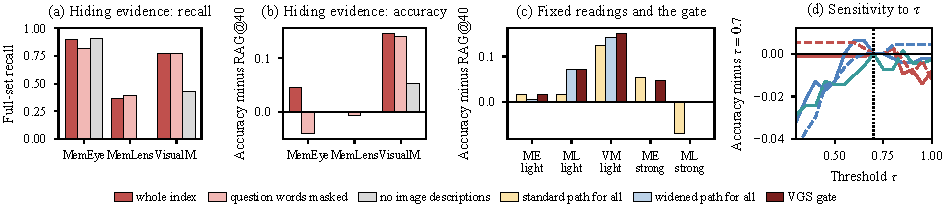
\includegraphics[width=\textwidth]{figures/gate.pdf}
\caption{(a,~b)~Full-set recall of \qss{} and its accuracy minus that of top-40 retrieval with the whole index, with every question word masked in the index lines, and without image descriptions in the index lines (MemEye: lightweight reader with thinking, the last bar from selection only; MemLens: test split; VisualMem: 150 random questions). (c)~Each reading applied to every question, and the gate, as accuracy minus top-40 retrieval with the same reader (ME: MemEye, ML: MemLens, VM: VisualMem). (d)~Accuracy of the gate as a function of the threshold $\tau$, relative to $\tau{=}0.7$ (red: MemEye, blue: MemLens, teal: VisualMem; solid: lightweight reader, dashed: strong reader). MemEye and VisualMem with the lightweight reader use the run of Table~\ref{tab:ablation}.}
\label{fig:vis}
\end{figure*}

Navigation can only reach what the index represents (Figure~\ref{fig:vis}a,b). Removing the image descriptions from the VisualMem index lowers the full-set recall of \qss{} from 0.773 to 0.433, the recall of top-40 retrieval, and its accuracy by 9.3 points $[4.0, 15.3]$. Masking the question words in the index lines, which leaves the evidence described, hurts only on MemEye: recall falls from 0.903 to 0.814, and the accuracy lead over top-40 retrieval turns from $+4.5$ into $-4.1$ points. On MemLens and VisualMem, masking does not lower recall ($+0.032$ and $0.000$). Index visibility, the share of question words in the evidence that the index lines show, is high on MemEye (95\%), intermediate on VisualMem (77\%), and low on MemLens (37\%), where the evidence is often an aside beyond the first 200 characters of a long message; the gate uses its estimate as a cheap signal of whether the index exposes the evidence.

The gate turns this condition into a choice of reading (Figure~\ref{fig:vis}c). Each fixed reading fails somewhere: for the lightweight reader, the standard path loses 5.3 points against the widened path on MemLens, and the widened path loses 1.2 points on MemEye; for the strong reader, set selection falls 7.1 points below wide retrieval on MemLens, and wide retrieval gives up 5.4 points on MemEye. The gate matches the better reading on every benchmark and reader and exceeds both on VisualMem (0.601 against 0.575 and 0.592). For the lightweight reader, it is also more accurate than a gate on message length with a threshold chosen the same way (by 0.6 to 1.8 points) and than random routing with the same share, and for both readers its accuracy stays within one point for thresholds between 0.6 and 0.8 (Figure~\ref{fig:vis}d). Within a benchmark, $\hat v(q)$ predicts only weakly which questions gain from the widened path (AUC 0.46 to 0.61; Appendix~\ref{app:vis}).

\subsection{Navigation Is Practical}
\label{sec:res-cost}

\begin{figure*}[t]
\centering
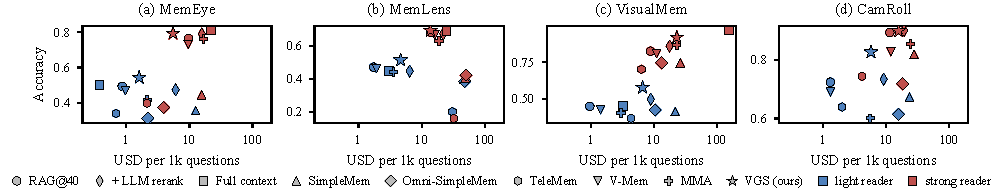
\includegraphics[width=\textwidth]{figures/cost.pdf}
\caption{(a--c)~Accuracy against cost per 1,000 questions on the question sets of Table~\ref{tab:main}, including memory construction and caches. (d)~Accuracy on MemEye against the median latency per question (Appendix~\ref{app:latency}). Markers distinguish methods and colors distinguish readers.}
\label{fig:cost}
\end{figure*}

Figure~\ref{fig:cost} places each method by accuracy, cost, and latency. On a persistent memory the index is static, so \vgs{} serves it from an explicit context cache: on MemEye, the cache lowers the cost of a selection call from \$9.4 to \$1.76 per 1,000 questions, and the strong reader with \vgs{} is both more accurate and cheaper than with top-40 retrieval (\$6.21 against \$9.78), since it reads seven selected rounds instead of 40. Long histories cost more: the VisualMem index has 99k tokens, so \vgs{} costs \$13.70 per 1,000 questions with the lightweight reader against \$0.96 for retrieval. Compacting the index lines, rather than bounding the index by similarity, keeps navigation over the whole history at a lower cost: in the run of Table~\ref{tab:ablation_full}, the compact index nearly halves the cost of \vgs{} on VisualMem (\$6.4 against \$11.7 per 1,000 questions, caches included) and keeps most of its gain ($+0.129$ against $+0.151$ over retrieval), whereas a 100-round pool costs about as much as the cached whole index (\$10.1) and keeps only half of the gain ($+0.078$). Latency stays close to retrieval: \vgs{} adds one selection call of 4 to 7~s but reads fewer rounds, so its median latency with the lightweight reader is 6.3~s against 5.4~s for top-40 retrieval on MemEye, and lower on MemLens and VisualMem (14.1 and 12.7~s against 16.5 and 15.7~s), where reading 40 long or image-rich rounds dominates.
